% !TeX encoding = GBK
\documentclass[journal, a4paper]{IEEEtran}
% some very useful LaTeX packages include:

%\usepackage{cite}      % Written by Donald Arseneau
                        % V1.6 and later of IEEEtran pre-defines the format
                        % of the cite.sty package \cite{} output to follow
                        % that of IEEE. Loading the cite package will
                        % result in citation numbers being automatically
                        % sorted and properly "ranged". i.e.,
                        % [1], [9], [2], [7], [5], [6]
                        % (without using cite.sty)
                        % will become:
                        % [1], [2], [5]--[7], [9] (using cite.sty)
                        % cite.sty's \cite will automatically add leading
                        % space, if needed. Use cite.sty's noadjust option
                        % (cite.sty V3.8 and later) if you want to turn this
                        % off. cite.sty is already installed on most LaTeX
                        % systems. The latest version can be obtained at:
                        % http://www.ctan.org/tex-archive/macros/latex/contrib/supported/cite/

\usepackage{graphicx}   % Written by David Carlisle and Sebastian Rahtz
                        % Required if you want graphics, photos, etc.
                        % graphicx.sty is already installed on most LaTeX
                        % systems. The latest version and documentation can
                        % be obtained at:
                        % http://www.ctan.org/tex-archive/macros/latex/required/graphics/
                        % Another good source of documentation is "Using
                        % Imported Graphics in LaTeX2e" by Keith Reckdahl
                        % which can be found as esplatex.ps and epslatex.pdf
                        % at: http://www.ctan.org/tex-archive/info/

%\usepackage{psfrag}    % Written by Craig Barratt, Michael C. Grant,
                        % and David Carlisle
                        % This package allows you to substitute LaTeX
                        % commands for text in imported EPS graphic files.
                        % In this way, LaTeX symbols can be placed into
                        % graphics that have been generated by other
                        % applications. You must use latex->dvips->ps2pdf
                        % workflow (not direct pdf output from pdflatex) if
                        % you wish to use this capability because it works
                        % via some PostScript tricks. Alternatively, the====+++
                        % graphics could be processed as separate files via
                        % psfrag and dvips, then converted to PDF for
                        % inclusion in the main file which uses pdflatex.
                        % Docs are in "The PSfrag System" by Michael C. Grant
                        % and David Carlisle. There is also some information
                        % about using psfrag in "Using Imported Graphics in
                        % LaTeX2e" by Keith Reckdahl which documents the
                        % graphicx package (see above). The psfrag package
                        % and documentation can be obtained at:
                        % http://www.ctan.org/tex-archive/macros/latex/contrib/supported/psfrag/

%\usepackage{subfigure} % Written by Steven Douglas Cochran
                        % This package makes it easy to put subfigures
                        % in your figures. i.e., "figure 1a and 1b"
                        % Docs are in "Using Imported Graphics in LaTeX2e"
                        % by Keith Reckdahl which also documents the graphicx
                        % package (see above). subfigure.sty is already
                        % installed on most LaTeX systems. The latest version
                        % and documentation can be obtained at:
                        % http://www.ctan.org/tex-archive/macros/latex/contrib/supported/subfigure/
%\usepackage[hidelinks]{hyperref}
\usepackage{hyperref}

%\usepackage{url}        % Written by Donald Arseneau
                        % Provides better support for handling and breaking
                        % URLs. url.sty is already installed on most LaTeX
                        % systems. The latest version can be obtained at:
                        % http://www.ctan.org/tex-archive/macros/latex/contrib/other/misc/
                        % Read the url.sty source comments for usage information.

%\usepackage{stfloats}  % Written by Sigitas Tolusis
                        % Gives LaTeX2e the ability to do double column
                        % floats at the bottom of the page as well as the top.
                        % (e.g., "\begin{figure*}[!b]" is not normally
                        % possible in LaTeX2e). This is an invasive package
                        % which rewrites many portions of the LaTeX2e output
                        % routines. It may not work with other packages that
                        % modify the LaTeX2e output routine and/or with other
                        % versions of LaTeX. The latest version and
                        % documentation can be obtained at:
                        % http://www.ctan.org/tex-archive/macros/latex/contrib/supported/sttools/
                        % Documentation is contained in the stfloats.sty
                        % comments as well as in the presfull.pdf file.
                        % Do not use the stfloats baselinefloat ability as
                        % IEEE does not allow \baselineskip to stretch.
                        % Authors submitting work to the IEEE should note
                        % that IEEE rarely uses double column equations and
                        % that authors should try to avoid such use.
                        % Do not be tempted to use the cuted.sty or
                        % midfloat.sty package (by the same author) as IEEE
                        % does not format its papers in such ways.

\usepackage{amsmath}    % From the American Mathematical Society
                        % A popular package that provides many helpful commands
                        % for dealing with mathematics. Note that the AMSmath
                        % package sets \interdisplaylinepenalty to 10000 thus
                        % preventing page breaks from occurring within multiline
                        % equations. Use:
%\interdisplaylinepenalty=2500
                        % after loading amsmath to restore such page breaks
                        % as IEEEtran.cls normally does. amsmath.sty is already
                        % installed on most LaTeX systems. The latest version
                        % and documentation can be obtained at:
                        % http://www.ctan.org/tex-archive/macros/latex/required/amslatex/math/
\hypersetup{
	colorlinks=true,
	linkcolor=black,
	urlcolor=red
}


% Other popular packages for formatting tables and equations include:

%\usepackage{array}
% Frank Mittelbach's and David Carlisle's array.sty which improves the
% LaTeX2e array and tabular environments to provide better appearances and
% additional user controls. array.sty is already installed on most systems.
% The latest version and documentation can be obtained at:
% http://www.ctan.org/tex-archive/macros/latex/required/tools/

% V1.6 of IEEEtran contains the IEEEeqnarray family of commands that can
% be used to generate multiline equations as well as matrices, tables, etc.

% Also of notable interest:
% Scott Pakin's eqparbox package for creating (automatically sized) equal
% width boxes. Available:
% http://www.ctan.org/tex-archive/macros/latex/contrib/supported/eqparbox/

% *** Do not adjust lengths that control margins, column widths, etc. ***
% *** Do not use packages that alter fonts (such as pslatex).         ***
% There should be no need to do such things with IEEEtran.cls V1.6 and later.


% Your document starts here!
\begin{document}
\begin{titlepage}

\newcommand{\HRule}{\rule{\linewidth}{0.5mm}} % Defines a new command for the horizontal lines, change thickness here

\center % Center everything on the page
 %----------------------------------------------------------------------------------------
%	LOGO SECTION
%----------------------------------------------------------------------------------------

~\\[1cm]

\includegraphics{SCUT.png}\\[2cm] % Include a department/university logo - this will require the graphicx package

%----------------------------------------------------------------------------------------
%	TITLE SECTION
%----------------------------------------------------------------------------------------

\HRule \\[1cm]
{ \huge \bfseries The Experiment Report of \textit{Machine Learning} }\\[0.6cm] % Title of your document
\HRule \\[2cm]
%----------------------------------------------------------------------------------------
%	HEADING SECTIONS
%----------------------------------------------------------------------------------------


\textsc{\LARGE \textbf{School:} School of Software Engineering}\\[1cm]
\textsc{\LARGE \textbf{Subject:} Software Engineering}\\[2cm] 

 
%----------------------------------------------------------------------------------------
%	AUTHOR SECTION
%----------------------------------------------------------------------------------------

\begin{minipage}{0.4\textwidth}
\begin{flushleft} \large
\emph{Author:}\\
ShiWangHua % Your name
\end{flushleft}
\end{minipage}
~
\begin{minipage}{0.4\textwidth}
\begin{flushright} \large
\emph{Supervisor:} \\
Mingkui Tan or Qingyao Wu % Supervisor's Name
\end{flushright}
\end{minipage}\\[2cm]
~
\begin{minipage}{0.4\textwidth}
\begin{flushleft} \large
\emph{Student ID:}\\
201630676843
\end{flushleft}
\end{minipage}
~
\begin{minipage}{0.4\textwidth}
\begin{flushright} \large
\emph{Grade:} \\
Undergraduate 
\end{flushright}
\end{minipage}\\[2cm]

% If you don't want a supervisor, uncomment the two lines below and remove the section above
%\Large \emph{Author:}\\
%John \textsc{Smith}\\[3cm] % Your name

%----------------------------------------------------------------------------------------
%	DATE SECTION
%----------------------------------------------------------------------------------------

{\large \today}\\[2cm] % Date, change the \today to a set date if you want to be precise

 
%----------------------------------------------------------------------------------------

\vfill % Fill the rest of the page with whitespace

\end{titlepage}

% Define document title and author
	\title{Face Detection Based on AdaBoost Algorithm}
	\maketitle

% Write abstract here
\begin{abstract}
In this experiment, there are two parts about face detection based on AdaBoost Algorithm. Our main task is among the first step which require to achieve the adaboost algorithm with the help of sklearn.tree library called DecisionTreeClassifier. Besides, preprocesssing of the data including extracting features from 1000 pictures is no small or negligible task.
\end{abstract}

% Each section begins with a \section{title} command
\section{Introduction}
\subsection{Problems}
The main problems to be solved within my reserarch are shown as below:
	\begin{quote}
	\begin{enumerate} 
	\item Extract NPD features correctly
	\item Achieve Adaboost by aid of DecisionTreeClassifier
	\item Adjust model, update parameters and improve the accuracy of the prediction
	\end{enumerate} 
    \end{quote}		
		
\subsection{Motivations}
	The motivations of this experiment are shown below:
	\begin{quote}
	\begin{enumerate} 
	\item Understand Adaboost algorithm further
	\item Get familiar with the basic method of face detection
	\item Learn to use Adaboost to solve the face detection problem, and combine the theory with the actual project
	\item Experience an complete process of machine learning
	\end{enumerate} 
    \end{quote}	
\subsection{Expectation}
	My expectation of this experiment have three points:
	\begin{quote}
		\begin{enumerate}
			\item Extract the features and save them to the local file
			\item Use adaboost algorithm and get an accuracy rate more than 0.9 on the given data set.
			\item Use OpenCV's build-in method based on Haar feature to achieve face detection 
		\end{enumerate}
	\end{quote}
\par

% Main Part
\section{Methods and Theory}
\subsection{Extract NPD features}
We can use this expression to create a NPD table(256*256):
 \begin{equation}
	\boldsymbol{table}[i][j]=(i-j)/(i+j)
 \end{equation}
The table is initialized to zero before calculating the formula above.
\par 
Then we can extract NPD features by this formula:
\begin{equation}
		\boldsymbol{features}[k]=	\boldsymbol{table}[	\boldsymbol{image}[i]][	\boldsymbol{image}[j]]
\end{equation}
In this formula, the 	$\boldsymbol{features}$ is a one dimension array(1*165600) in which the 165600 menans 576 plus 575 then divide by 2 and the 576 means the number of image's pixels. The 	$\boldsymbol{image}$ is a one dimension array storing the value of pixels.\par
\subsection{Calculate the error rate $\boldsymbol{\epsilon}$}
Error rate $\boldsymbol{\epsilon}$ is used to evaluate the accuracy of the output of weak classifiers. For any $\boldsymbol{y}$ predicted by weak classifier which is not equal to the actual $\boldsymbol{y}$ value, we can get a cumulative sum of all the $\boldsymbol{w}$ (a w value means the weight of a sample) in corresponding  $\boldsymbol{y}$'s position. Then we use the cumulative sum as error rate $\boldsymbol{\epsilon}$. This calculation can be expressed in mathmatical formula as follows:
\begin{equation}
	\boldsymbol{\epsilon}_m=\sum_{i=1}^N \boldsymbol{w}_\mathrm{(m,i)}II(y_i\ne h_m(x_i))
\end{equation}
In this formula, the m means the number of weak classifier, N means the number of samples whcih equal to 1000, and $h_m(x_i)$ means the predict value $\boldsymbol{y}$. If the prediction is wrong, $II(y_i\ne h_m(x_i))$ is equal to 1.
\par 

\subsection{Update weak classifier's weight $\boldsymbol{\alpha}$}
To calculate $\alpha$, we need to calculate the derivation of the weighted exponential loss and set the derivation as zero. The final loss we work out is:
\begin{equation}
	\boldsymbol{L}(\boldsymbol{y},\boldsymbol{h}_m(\boldsymbol{x}))=e^{-\alpha_m} (1-\epsilon_m)+e^\alpha_m \epsilon_m
\end{equation} 
Calculate the derivation of (4):
\begin{equation}
	 \frac{\partial \boldsymbol{L}(\boldsymbol{y},\boldsymbol{h}_m(\boldsymbol{x}))}{\partial \alpha_m}=-e^{-\alpha_m}(1-\epsilon_m)+e^{\alpha_m}\epsilon_m
\end{equation}
Set (5) as zero, we finally get the expression of $\alpha_m$:
\begin{equation}
	\alpha_m= \frac{1}{2}log_2 \frac{1-\epsilon_m}{\epsilon_m}
\end{equation}

\subsection{Update sample weight $\boldsymbol{w}$}
Based on $\boldsymbol{F}_m(x)=\boldsymbol{F}_{m-1}(x)+\alpha_m\boldsymbol{h}_m(x)$, we can finally get the update equationof w:
\begin{equation}
	w_{(m+1,i)}=\frac{w_{(m,i)}e^{-y_i\alpha_mh_m(x_i)}}{z_m}
\end{equation}
where $z_m=\sum_{i=1}^Nw_{(m,i)}e^{-y_i\alpha_mh_m(x_i)}$ aims to renormalization.
%In this section, you are asked to give a complete introduction to the experiment. For instance, the chosen methods, the related theories, the related equations(loss function), the derivation process(taking the gradient) and so on.

\section{Experiments}
\subsection{Dataset}
\begin{enumerate}
	\item This experiment provides 1000 pictures, of which 500 are human face RGB images, stored in datasets/original/face; the other 500 are non-face RGB images, stored in datasets/original/nonface.
	\item The dataset is included in the \href{https://github.com/wujiaju/ML2018-lab-03}{example repository}. We need to divide it into training set and validation set.
\end{enumerate}

\subsection{Implementation}
%All detailed implementation in your experiment: initialization, process, results, all kinds of parameters. In a word, describe clearly What you do and how you do.\par
%\subparagraph{Face Classification}
\begin{itemize}
	\item Face Classification
%\subsubsection{Face Classification}
\begin{enumerate}
	\item Load data set and read them into memory. Use $\boldsymbol{Image.open.convert}$ to convert the images to grayscale images with size of 24 * 24.
	\item Process data set: extract NPD features using the NPDFeature class in feature.py. 
	\item Use $\boldsymbol{sklearn.model\_selection.train\_test\_split}$ to divide the data set into training set and validation set.
	\item Write all AdaBoostClassifier functions based on the reserved interface in ensemble.py according to part II.
	\item Predict and verify the accuracy on the validation set using the method in AdaBoostClassifier. Use classification\_report() of the $\boldsymbol{sklearn.metrics}$ library function to write predicted result to $\boldsymbol{classifier\_report.txt}$.
\end{enumerate}
   \item Face Detection
   \begin{enumerate}
   	\item Run the "face\_detection.py" file. Experience the OpenCV's built-in method of face detection using Haar Feature-based Cascade Classifiers.The result will be save as detect\_result.jpg.
   	\item Use other images to replace the default test image.
   \end{enumerate}
\end{itemize}
	% You can reference tables and figure by using the \ref{label} command. Each table and figure needs to have a UNIQUE label.

	% This is how you define a table: the [!hbt] means that LaTeX is forced (by the !) to place the table exactly here (by h), or if that doesnt work because of a pagebreak or so, it tries to place the table to the bottom of the page (by b) or the top (by t).

	% If you have questions about how to write mathematical formulas in LaTeX, please read a LaTeX book or the 'Not So Short Introduction to LaTeX': tobi.oetiker.ch/lshort/lshort.pdf

	% This is how you include a eps figure in your document. LaTeX only accepts EPS or TIFF files.


\section{Conclusion}
	The ouput is shown in Fig.~\ref{fig:tf_plot}. We can see the accuracy is about 90\%.
	\begin{figure}[!hbt]
	% Center the figure.
	\begin{center}
		% Include the eps file, scale it such that it's width equals the column width. You can also put width=8cm for example...
		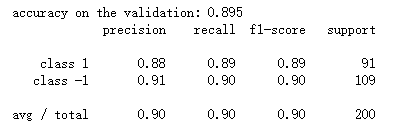
\includegraphics[width=\columnwidth]{result}
		% Create a subtitle for the figure.
		\centering
		\caption{\quad Classification Report of Face Detection}
		% Define the label of the figure. It's good to use 'fig:title', so you know that the label belongs to a figure.
		\label{fig:tf_plot}
	\end{center}
	\end{figure}
\par
By this expriment, I learned a lot about machine learning and experience an complete process of machine learning. Besides, this is my first time to write an experiment report using latex, which makes me gain another useful skill for my personal dedvelopment. Thanks to teacher Mr.Tan and assistants a lot ! 

% Your document ends here!
\end{document}